\documentclass[twoside]{book}

% Packages required by doxygen
\usepackage{fixltx2e}
\usepackage{calc}
\usepackage{doxygen}
\usepackage[export]{adjustbox} % also loads graphicx
\usepackage{graphicx}
\usepackage[utf8]{inputenc}
\usepackage{makeidx}
\usepackage{multicol}
\usepackage{multirow}
\PassOptionsToPackage{warn}{textcomp}
\usepackage{textcomp}
\usepackage[nointegrals]{wasysym}
\usepackage[table]{xcolor}

% Font selection
\usepackage[T1]{fontenc}
\usepackage[scaled=.90]{helvet}
\usepackage{courier}
\usepackage{amssymb}
\usepackage{sectsty}
\renewcommand{\familydefault}{\sfdefault}
\allsectionsfont{%
  \fontseries{bc}\selectfont%
  \color{darkgray}%
}
\renewcommand{\DoxyLabelFont}{%
  \fontseries{bc}\selectfont%
  \color{darkgray}%
}
\newcommand{\+}{\discretionary{\mbox{\scriptsize$\hookleftarrow$}}{}{}}

% Page & text layout
\usepackage{geometry}
\geometry{%
  a4paper,%
  top=2.5cm,%
  bottom=2.5cm,%
  left=2.5cm,%
  right=2.5cm%
}
\tolerance=750
\hfuzz=15pt
\hbadness=750
\setlength{\emergencystretch}{15pt}
\setlength{\parindent}{0cm}
\setlength{\parskip}{3ex plus 2ex minus 2ex}
\makeatletter
\renewcommand{\paragraph}{%
  \@startsection{paragraph}{4}{0ex}{-1.0ex}{1.0ex}{%
    \normalfont\normalsize\bfseries\SS@parafont%
  }%
}
\renewcommand{\subparagraph}{%
  \@startsection{subparagraph}{5}{0ex}{-1.0ex}{1.0ex}{%
    \normalfont\normalsize\bfseries\SS@subparafont%
  }%
}
\makeatother

% Headers & footers
\usepackage{fancyhdr}
\pagestyle{fancyplain}
\fancyhead[LE]{\fancyplain{}{\bfseries\thepage}}
\fancyhead[CE]{\fancyplain{}{}}
\fancyhead[RE]{\fancyplain{}{\bfseries\leftmark}}
\fancyhead[LO]{\fancyplain{}{\bfseries\rightmark}}
\fancyhead[CO]{\fancyplain{}{}}
\fancyhead[RO]{\fancyplain{}{\bfseries\thepage}}
\fancyfoot[LE]{\fancyplain{}{}}
\fancyfoot[CE]{\fancyplain{}{}}
\fancyfoot[RE]{\fancyplain{}{\bfseries\scriptsize Generated by Doxygen }}
\fancyfoot[LO]{\fancyplain{}{\bfseries\scriptsize Generated by Doxygen }}
\fancyfoot[CO]{\fancyplain{}{}}
\fancyfoot[RO]{\fancyplain{}{}}
\renewcommand{\footrulewidth}{0.4pt}
\renewcommand{\chaptermark}[1]{%
  \markboth{#1}{}%
}
\renewcommand{\sectionmark}[1]{%
  \markright{\thesection\ #1}%
}

% Indices & bibliography
\usepackage{natbib}
\usepackage[titles]{tocloft}
\setcounter{tocdepth}{3}
\setcounter{secnumdepth}{5}
\makeindex

% Hyperlinks (required, but should be loaded last)
\usepackage{ifpdf}
\ifpdf
  \usepackage[pdftex,pagebackref=true]{hyperref}
\else
  \usepackage[ps2pdf,pagebackref=true]{hyperref}
\fi
\hypersetup{%
  colorlinks=true,%
  linkcolor=blue,%
  citecolor=blue,%
  unicode%
}

% Custom commands
\newcommand{\clearemptydoublepage}{%
  \newpage{\pagestyle{empty}\cleardoublepage}%
}

\usepackage{caption}
\captionsetup{labelsep=space,justification=centering,font={bf},singlelinecheck=off,skip=4pt,position=top}

%===== C O N T E N T S =====

\begin{document}

% Titlepage & ToC
\hypersetup{pageanchor=false,
             bookmarksnumbered=true,
             pdfencoding=unicode
            }
\pagenumbering{roman}
\begin{titlepage}
\vspace*{7cm}
\begin{center}%
{\Large Simple I\+EC 61850 Server }\\
\vspace*{1cm}
{\large Generated by Doxygen 1.8.11}\\
\end{center}
\end{titlepage}
\clearemptydoublepage
\tableofcontents
\clearemptydoublepage
\pagenumbering{arabic}
\hypersetup{pageanchor=true}

%--- Begin generated contents ---
\chapter{File Index}
\section{File List}
Here is a list of all documented files with brief descriptions\+:\begin{DoxyCompactList}
\item\contentsline{section}{src/\hyperlink{simple-iec61850-client_8c}{simple-\/iec61850-\/client.\+c} \\*Test Class }{\pageref{simple-iec61850-client_8c}}{}
\end{DoxyCompactList}

\chapter{File Documentation}
\hypertarget{simple-iec61850-server_8c}{}\section{src/simple-\/iec61850-\/server.c File Reference}
\label{simple-iec61850-server_8c}\index{src/simple-\/iec61850-\/server.\+c@{src/simple-\/iec61850-\/server.\+c}}


Simple I\+EC 61850 Server.  


{\ttfamily \#include \char`\"{}iec61850\+\_\+server.\+h\char`\"{}}\\*
{\ttfamily \#include \char`\"{}hal\+\_\+thread.\+h\char`\"{}}\\*
{\ttfamily \#include $<$signal.\+h$>$}\\*
{\ttfamily \#include $<$stdlib.\+h$>$}\\*
{\ttfamily \#include $<$stdio.\+h$>$}\\*
{\ttfamily \#include \char`\"{}argp.\+h\char`\"{}}\\*
{\ttfamily \#include \char`\"{}static\+\_\+model.\+h\char`\"{}}\\*
Include dependency graph for simple-\/iec61850-\/server.c\+:
\nopagebreak
\begin{figure}[H]
\begin{center}
\leavevmode
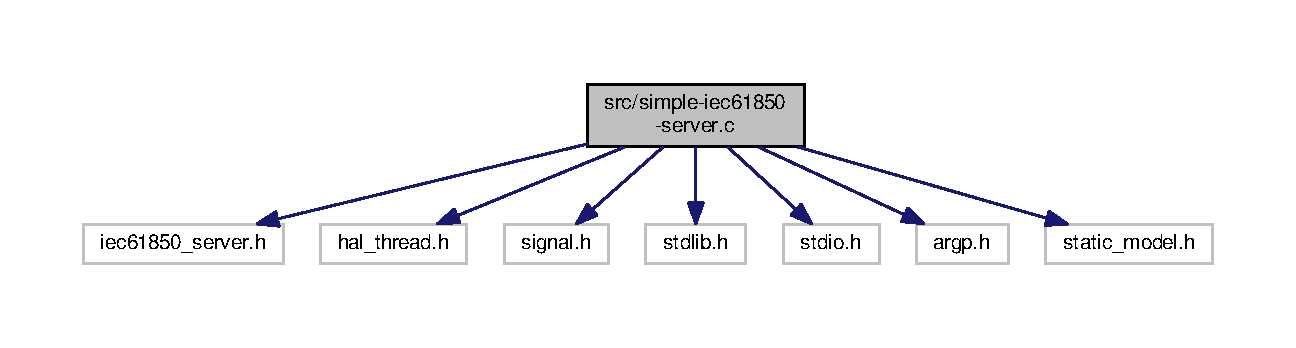
\includegraphics[width=350pt]{simple-iec61850-server_8c__incl}
\end{center}
\end{figure}
\subsection*{Functions}
\begin{DoxyCompactItemize}
\item 
void \hyperlink{simple-iec61850-server_8c_aa0bd1ed4ed81822b72a2b4fb9acba63f}{sigint\+\_\+handler} (int signal\+Id)\hypertarget{simple-iec61850-server_8c_aa0bd1ed4ed81822b72a2b4fb9acba63f}{}\label{simple-iec61850-server_8c_aa0bd1ed4ed81822b72a2b4fb9acba63f}

\begin{DoxyCompactList}\small\item\em Function to implement signal handler for abort. \end{DoxyCompactList}\item 
void \hyperlink{simple-iec61850-server_8c_ab704e21febb6ba6f62fd7182fabea02b}{run\+Server} ()\hypertarget{simple-iec61850-server_8c_ab704e21febb6ba6f62fd7182fabea02b}{}\label{simple-iec61850-server_8c_ab704e21febb6ba6f62fd7182fabea02b}

\begin{DoxyCompactList}\small\item\em Function for running the server. \end{DoxyCompactList}\item 
static int \hyperlink{simple-iec61850-server_8c_aaf7bc24f3891f0c63a6043f4dc2ab311}{parse\+\_\+opt} (int key, char $\ast$arg, struct argp\+\_\+state $\ast$state)
\begin{DoxyCompactList}\small\item\em Function which parses the given options and arguments. \end{DoxyCompactList}\item 
int \hyperlink{simple-iec61850-server_8c_a3c04138a5bfe5d72780bb7e82a18e627}{main} (int argc, char $\ast$$\ast$argv)
\begin{DoxyCompactList}\small\item\em Main function. \end{DoxyCompactList}\end{DoxyCompactItemize}
\subsection*{Variables}
\begin{DoxyCompactItemize}
\item 
const char $\ast$ \hyperlink{simple-iec61850-server_8c_a62f73ea01c816f1996aed4c66f57c4fb}{argp\+\_\+program\+\_\+version} = \char`\"{}Simple I\+EC 61850 Server version 1.\+0.\+0\char`\"{}
\begin{DoxyCompactList}\small\item\em Global variable for the version. \end{DoxyCompactList}\item 
Ied\+Model {\bfseries ied\+Model}\hypertarget{simple-iec61850-server_8c_a12458534e574afa1fd44b76a5b691719}{}\label{simple-iec61850-server_8c_a12458534e574afa1fd44b76a5b691719}

\item 
static int \hyperlink{simple-iec61850-server_8c_a2f45113638a0b749a8a205d2cd7fb42b}{running} = 0\hypertarget{simple-iec61850-server_8c_a2f45113638a0b749a8a205d2cd7fb42b}{}\label{simple-iec61850-server_8c_a2f45113638a0b749a8a205d2cd7fb42b}

\begin{DoxyCompactList}\small\item\em Global variable for state of server. \end{DoxyCompactList}\item 
int \hyperlink{simple-iec61850-server_8c_ac31354d08316076b496efb2b3a2c69e6}{tcp\+Port} = 10102\hypertarget{simple-iec61850-server_8c_ac31354d08316076b496efb2b3a2c69e6}{}\label{simple-iec61850-server_8c_ac31354d08316076b496efb2b3a2c69e6}

\begin{DoxyCompactList}\small\item\em Global variable for tcp port. \end{DoxyCompactList}\item 
float \hyperlink{simple-iec61850-server_8c_af2eae6b68aca1a3174f57157c50f58f1}{power} = 500.f\hypertarget{simple-iec61850-server_8c_af2eae6b68aca1a3174f57157c50f58f1}{}\label{simple-iec61850-server_8c_af2eae6b68aca1a3174f57157c50f58f1}

\begin{DoxyCompactList}\small\item\em Global variable for the the default value of the power. \end{DoxyCompactList}\item 
int \hyperlink{simple-iec61850-server_8c_af40caf0f193ce7061522488c9df48f02}{is\+Verbose} = 0\hypertarget{simple-iec61850-server_8c_af40caf0f193ce7061522488c9df48f02}{}\label{simple-iec61850-server_8c_af40caf0f193ce7061522488c9df48f02}

\begin{DoxyCompactList}\small\item\em Global variable for verbose output. \end{DoxyCompactList}\end{DoxyCompactItemize}


\subsection{Detailed Description}
Simple I\+EC 61850 Server. 

This C-\/\+File implements a simple I\+EC 61850 client. The library lib\+I\+E\+C61850 is used for implementing the protocol I\+EC 61850. Argp is used to parse the options and arguments from the command line.

\begin{DoxyAuthor}{Author}
David Mittelstädt 
\end{DoxyAuthor}
\begin{DoxySeeAlso}{See also}
\href{https://github.com/dmittelstaedt/siprenz-protocols}{\tt https\+://github.\+com/dmittelstaedt/siprenz-\/protocols} 

\href{http://libiec61850.com/libiec61850/}{\tt http\+://libiec61850.\+com/libiec61850/} 
\end{DoxySeeAlso}


\subsection{Function Documentation}
\index{simple-\/iec61850-\/server.\+c@{simple-\/iec61850-\/server.\+c}!main@{main}}
\index{main@{main}!simple-\/iec61850-\/server.\+c@{simple-\/iec61850-\/server.\+c}}
\subsubsection[{\texorpdfstring{main(int argc, char $\ast$$\ast$argv)}{main(int argc, char **argv)}}]{\setlength{\rightskip}{0pt plus 5cm}int main (
\begin{DoxyParamCaption}
\item[{int}]{argc, }
\item[{char $\ast$$\ast$}]{argv}
\end{DoxyParamCaption}
)}\hypertarget{simple-iec61850-server_8c_a3c04138a5bfe5d72780bb7e82a18e627}{}\label{simple-iec61850-server_8c_a3c04138a5bfe5d72780bb7e82a18e627}


Main function. 

Starts the parsing function and then starts the server 
\begin{DoxyParams}{Parameters}
{\em argc} & Number of arguments \\
\hline
{\em argv} & Content of the arguments \\
\hline
\end{DoxyParams}
\begin{DoxyReturn}{Returns}
Exit status of the application 
\end{DoxyReturn}
\index{simple-\/iec61850-\/server.\+c@{simple-\/iec61850-\/server.\+c}!parse\+\_\+opt@{parse\+\_\+opt}}
\index{parse\+\_\+opt@{parse\+\_\+opt}!simple-\/iec61850-\/server.\+c@{simple-\/iec61850-\/server.\+c}}
\subsubsection[{\texorpdfstring{parse\+\_\+opt(int key, char $\ast$arg, struct argp\+\_\+state $\ast$state)}{parse_opt(int key, char *arg, struct argp_state *state)}}]{\setlength{\rightskip}{0pt plus 5cm}static int parse\+\_\+opt (
\begin{DoxyParamCaption}
\item[{int}]{key, }
\item[{char $\ast$}]{arg, }
\item[{struct argp\+\_\+state $\ast$}]{state}
\end{DoxyParamCaption}
)\hspace{0.3cm}{\ttfamily [static]}}\hypertarget{simple-iec61850-server_8c_aaf7bc24f3891f0c63a6043f4dc2ab311}{}\label{simple-iec61850-server_8c_aaf7bc24f3891f0c63a6043f4dc2ab311}


Function which parses the given options and arguments. 

Function to parse the given options and arguments with the help of argp. 
\begin{DoxyParams}{Parameters}
{\em key} & Key for identifying \\
\hline
{\em arg} & Value of the key \\
\hline
{\em state} & Struct \\
\hline
\end{DoxyParams}
\begin{DoxyReturn}{Returns}
Return code of parsing the arguments 
\end{DoxyReturn}


\subsection{Variable Documentation}
\index{simple-\/iec61850-\/server.\+c@{simple-\/iec61850-\/server.\+c}!argp\+\_\+program\+\_\+version@{argp\+\_\+program\+\_\+version}}
\index{argp\+\_\+program\+\_\+version@{argp\+\_\+program\+\_\+version}!simple-\/iec61850-\/server.\+c@{simple-\/iec61850-\/server.\+c}}
\subsubsection[{\texorpdfstring{argp\+\_\+program\+\_\+version}{argp_program_version}}]{\setlength{\rightskip}{0pt plus 5cm}const char$\ast$ argp\+\_\+program\+\_\+version = \char`\"{}Simple I\+EC 61850 Server version 1.\+0.\+0\char`\"{}}\hypertarget{simple-iec61850-server_8c_a62f73ea01c816f1996aed4c66f57c4fb}{}\label{simple-iec61850-server_8c_a62f73ea01c816f1996aed4c66f57c4fb}


Global variable for the version. 

This variable is used from argp to set the output for the version option. 
%--- End generated contents ---

% Index
\backmatter
\newpage
\phantomsection
\clearemptydoublepage
\addcontentsline{toc}{chapter}{Index}
\printindex

\end{document}
